\documentclass{article}
\usepackage{geometry}
\geometry{a4paper, top=3cm, bottom=3cm, left=3.5cm, right=3.5cm, heightrounded, bindingoffset=5mm}

%\documentclass[12pt, letterpaper, twoside]{article}
\usepackage[utf8]{inputenc}

\renewcommand{\contentsname}{Indice}

\usepackage{algpseudocode}
\usepackage{hyperref}
\usepackage{amsmath}
\usepackage{caption}
\usepackage{float}
\usepackage{enumitem}
\hypersetup{hidelinks}
% Sillabazione italiana
\usepackage[italian]{babel}
%\usepackage{authblk}
% Json format
%\usepackage{bera}% optional: just to have a nice mono-spaced font
\usepackage{listings}
\usepackage{xcolor}

\usepackage{multirow}


\usepackage{graphicx}
\graphicspath{ {./images/} }


\title{\textbf{Covid19 Fake News Detection} \\[1ex] \large Università degli Studi Roma Tre, Dipartimento di Ingegneria Informatica \\[1ex] \normalsize Progetto per il corso di Sistemi Intelligenti per Internet e Machine Learning}
\date{}

\begin{document}
\maketitle
\begin{flushleft}
\textbf{Manuel Granchelli} 
\hfill {\href{mailto:man.granchelli@stud.uniroma3.it}{\textbf{man.granchelli@stud.uniroma3.it}}} \\
\textit{Matricola: 512406}\\
\textbf{Alessandro Dell'Oste} 
\hfill {\href{mailto:ale.delloste@stud.uniroma3.it}{\textbf{ale.delloste@stud.uniroma3.it}}} \\
\textit{Matricola: 502589}\\


\par\bigskip
\textbf{Repo GitHub:} \href{https://github.com/mgranchelli/covid19-fake-news-detection} {https://github.com/mgranchelli/covid19-fake-news-detection}
\end{flushleft}

\section*{Introduzione}
L'uso dei social media è aumentato negli ultimi anni. Nel 2020 ci sono stati oltre 3,6 miliardi di utenti sui social media e entro il 2025 si prevede che ci saranno circa 4,41 miliardi di utenti. I social media hanno introdotto diversi benefici come rendere la comunicazione più rapida e semplice con persone di tutte il mondo, promuovere marchi, feedback dei clienti e notizie in tempo reale.
Tuttavia, presenta anche diversi svantaggi come mettere a rischio la propria privacy, ridurre il contatto personale e uno dei più importanti è la diffusione di informazioni false (fake news) e poco affidabili. 
In particolare, proprio quest'ultime sono diventate un problema molto impegnativo sui social, perchè, data la facilità e rapidità nella comunicazione, notizie false possono fare il giro del mondo in pochissimo tempo. Queste fake news sono semplici articoli (es: tweet, post) che vengono creati ad hoc per screditare un personaggio pubblico o manipolare la verità dei fatti di un evento. Infatti, nel 2020 con l'arrivo della pandemia da Covid-19, sui social sono dilagate notizie false dove si proponevano cure o nelle quali si affermava che la pandemia fosse solo una finzione. Ad esempio, la fake news \textit{"L'alcol è una cura per la COVID-19"} ha causato molti decessi e ricoveri in ospedale in Iran. Questo dimostra quanto si può essere vulnerabile dalle fake news e quanto gravi possano essere gli esiti se le ignoriamo.

\noindent
L'obiettivo del seguente progetto è stato quello di utilizzare tecniche di apprendimento automatico per classificare le notizie come vere o false. Le notizie sono limitate all'argomento della pandemia da Covid-19. Nel seguente caso è stato utilizzato un dataset contenente dati con affermazioni vere e false raccolti da vari siti e da social media. Il dataset utilizzato è presente nella competizione \textit{Constraint@AAAI2021 - COVID19 Fake News Detection in English} raggiungibile al seguente link: \href{https://competitions.codalab.org/competitions/26655} {\textit{https://competitions.codalab.org/}}. \\
I dati sono stati analizzati, visualizzati e ripuliti. In seguito, sono stati addestrati e testati cinque modelli di machine learning per la classificazione delle notizie.

\noindent
Il materiale utilizzato è presente su GitHub al seguente link: 

\noindent
\href{https://github.com/mgranchelli/covid19-fake-news-detection} {https://github.com/mgranchelli/covid19-fake-news-detection}.




\thispagestyle{empty}
\newpage

\tableofcontents

% Remove number page and start sections from this page
\thispagestyle{empty}

\clearpage
\pagenumbering{arabic}

\section{Analisi del dataset}
Per procedere al rilevamento di fake news relative al Covid-19, abbiamo utilizzato il dataset fornito ai partecipanti di \textbf{Constraint@AAAI2021 - COVID19 Fake News Detection in English}.
Il dataset contiene real e fake news in merito al Covid-19; i \textbf{real} sono tweet raccolti da sorgenti verificate e forniscono informazioni utili mentre i \textbf{fake} sono tweet, posts ed articoli verificati ma che non sono veri. La tabella 1 fornisce alcuni esempi estratti dal dataset.

\begin{table}[h]
\begin{center}
\begin{tabular}{| l | p{11cm} |}
\hline
\textbf{Label} & \textbf{Fake} \\
\hline
Real & Take simple daily precautions to help prevent the spread of respiratory illnesses like \#COVID19. Learn how to protect yourself from coronavirus (COVID-19): https://t.co/uArGZTrH5L. https://t.co/biZTxtUKyK \\
\hline
Fake & 'Politically Correct Woman (Almost) Uses Pandemic as Excuse Not to Reuse Plastic Bag https://t.co/thF8GuNFPe \#coronavirus \#nashville'  \\
\hline
Real & 'Take simple daily precautions to help prevent the spread of respiratory illnesses like \#COVID19. Learn how to protect yourself from coronavirus (COVID-19): https://t.co/uArGZTrH5L. https://t.co/biZTxtUKyK' \\
\hline
Fake & 'The NBA is poised to restart this month. In March we reported on how the Utah Jazz got 58 coronavirus tests in a matter of hours at a time when U.S. testing was sluggish. https://t.co/I8YjjrNoTh https://t.co/o0Nk6gpyos' \\
\hline
Real & 'We just announced that the first participants in each age cohort have been dosed in the Phase 2 study of our mRNA vaccine (mRNA-1273) against novel coronavirus. Read more: https://t.co/woPlKz1bZC \#mRNA https://t.co/9VGUoJu5cS' \\
\hline
Real & '\#CoronaVirusUpdates \#IndiaFightsCorona More than 6 lakh tests done for 3rd successive day. Cumulative testing as on date has reached 22149351. \#COVID19 Tests Per Million (TPM) cross 16000.' \\
\hline
\end{tabular}
\end{center}
\caption{Esempi di real e fake news del dataset}
\end{table}

\noindent
%Al fine di ottenere un dataset coerente, durante la fase di raccolta i tweet sono stati filtrati in lingua inglese il cui contenuto è legato al topic Covid-19.
I tweet presenti nel dataset sono in lingua inglese e il cui contenuto è legato sola al topic Covid-19.

\subsection{Fake news}
Le fake news sono state collezionate da siti web e social media e la loro veridicità è stata verificata manualmente attraverso documenti originali. Varie risorse come post di Facebook, tweet, post di Instagram, dichiarazioni pubbliche, comunicati stampa o altro contenuto multimediale sono state utilizzate per raccogliere fake news.

\subsection{Real news}
Sono stati collezionati tweet pubblicati da enti affidabili come governi, enti medici e testate scientifiche; ad esempio i tweet collezionati sono stati pubblicati da enti come \textit{World Health Organization (WHO)}, \textit{Centers for Disease Control and Prevention (CDC)}, ect. Ogni tweet è stato verificato manualmente ed identificato come real se contiene informazioni inerenti al Covid-19, ad esempio l'avanzamento del numero dei vaccinati, ect.

\subsection{Statistiche}

Dalla tabella 2, si osserva che in generale le real news sono più lunghe delle fake news sia in termini di parole che di caratteri per tweet. Le \textit{unique words} all'interno del dataset sono 18346 di cui 4289 parole sono condivise tra real e fake news.

\begin{table}[h]
\begin{center}
\begin{tabular}{| l | l | l | l |}
\hline
\textbf{Attribute} & \textbf{Fake} & \textbf{Real}  & \textbf{All}  \\
\hline
Unique words & 12122 & 10513 & 18346 \\
\hline
Avg words per post & 21.65 & 31.96 & 27.05 \\
\hline
Avg chars per post & 143.21 & 217.12 & 181.89 \\
\hline
\end{tabular}
\end{center}
\caption{Caratteristiche del dataset}
\end{table}

\noindent
Il dataset utilizzato è stato suddiviso in \textit{train} (60\%), \textit{validation} (20\%) e \textit{test} (20\%). La Figura 1 mostra la suddivisione dei dati per categoria.

\begin{figure}[H]
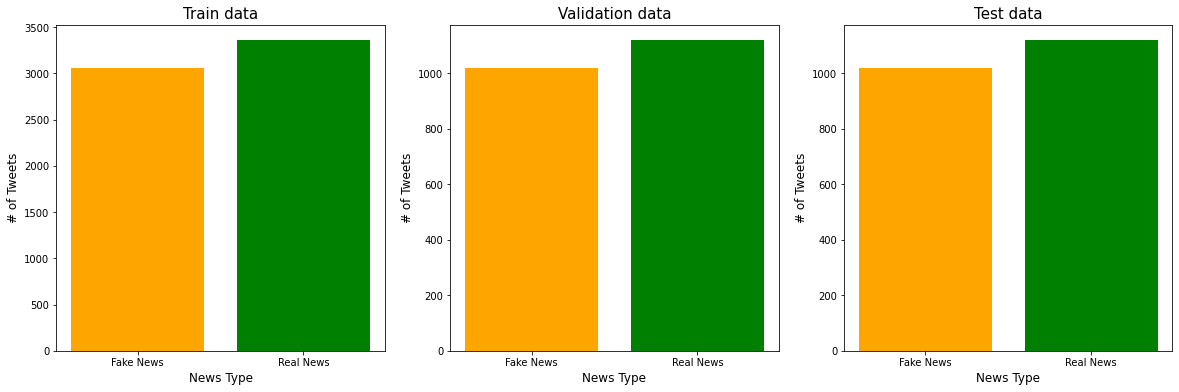
\includegraphics[width=1\linewidth]{dataset.png}
\centering
\caption{Distribuzione dei dati}
\label{fig:bytepost}
\end{figure}

\noindent
Il dataset risulta bilanciato in quanto circa il 52\% sono real news mentre circa il 48\% sono fake news.
Analizzando il dataset ed effettuando una classificazione \textit{token-level}, dopo aver rimosso le \textit{stopwords}, si ottengo i seguenti dieci token più frequenti:
\begin{itemize}[noitemsep]
  \item \textbf{Fake}: coronavirus, covid19, people, virus, trump, new, pandemic, vaccine, india, says.
  \item \textbf{Real}: covid19, cases, new, tests, deaths, total, states, number, people, confirmed.
  \item \textbf{All}: covid19, cases, coronavirus, new, people, tests, deaths, states, total, covid.
\end{itemize}

\noindent
Le Figure 2a, 2b ed 2c mostrano le word clouds per real, fake e all tweet. Analizzando le word cloud e le parole più frequenti, si può vedere come c'è una significativa sovrapposizione di parole tra real e fake news


\begin{figure}[H]
\minipage{0.32\textwidth}
  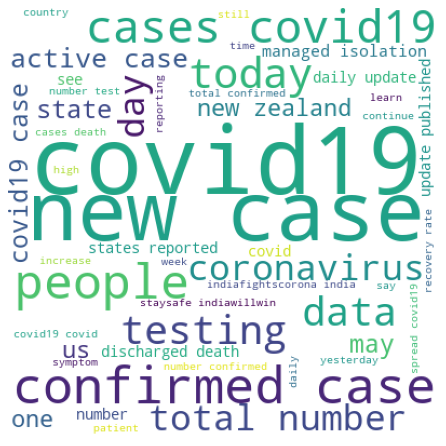
\includegraphics[width=\linewidth]{real_tokens.png}
  \caption*{(a) - Real Tokens}\label{fig:real_tokens}
\endminipage\hfill
\minipage{0.32\textwidth}
  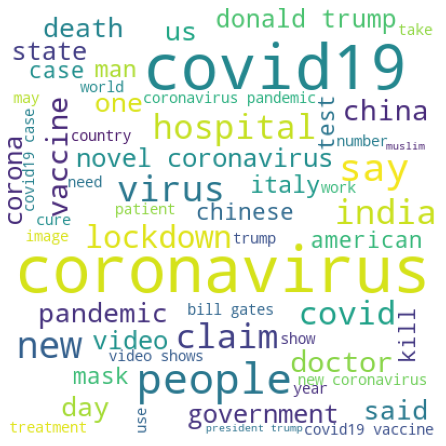
\includegraphics[width=\linewidth]{fake_tokens.png}
  \caption*{(b) - Fake Tokens}\label{fig:fake_tokens}
\endminipage\hfill
\minipage{0.32\textwidth}%
  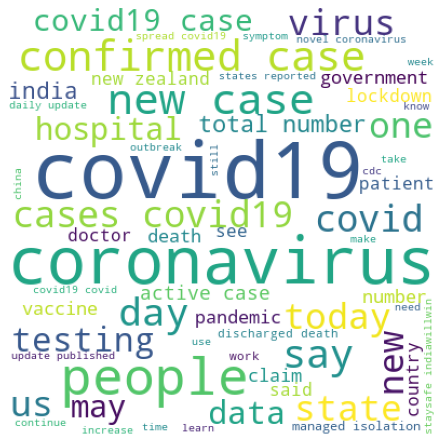
\includegraphics[width=\linewidth]{all_tokens.png}
  \caption*{(c) - All Tokens}\label{fig:all_tokens.png}
\endminipage
\caption{Word Clouds generato dal dataset}
\end{figure}







\newpage
\section{Modelli addestrati e risultati}
Il codice utilizzato per addestrare e testare i modelli di machine learning è presente all'interno del notebook \textit{fake-news-ml.ipynb} presente all'interno del \href{https://github.com/mgranchelli/covid19-fake-news-detection}{repo}. Il dataset a disposizione è composto da tre file da utilizzare per l'addestramento (train), la validazione (val) e il test (test) del modello. Una volta caricati i dati per ogni set di dati sono stati eliminati caratteri speciali, segni di punteggiatura e sono state rimosse tutte le stopwords. Per la rimozione delle stopwords è stata utilizzata la libreria \textit{nltk} e in particolare, siccome nel dataset sono presenti tweet in inglese, sono state importate solo le stopwords relative alla lingua inglese. Successivamente sono state convertite le label (real, fake) dei tweet in formato binario dove lo \texttt{0} corrisponde ad una \texttt{notizia falsa} e \texttt{1} ad una \texttt{notizia vera} ed è stato applicato tf-idf al testo dei tweet. \textbf{Tf-idf} è una funzione utilizzata per misurare l'importanza di un termine rispetto ad un documento o ad una collezione di documenti. In seguito, sono riportati i cinque modelli di machine learning applicati per la classificazione di notizie vere/false. Per mostrare i risultati delle metriche ottenute è stata utilizzata una funzione per stampare la matrice di confusione presente nel codice degli organizzatori della competizione da cui sono stati ottenuti i dati. La matrice di confusione restituisce una rappresentazione dell'accuratezza di classificazione. Inoltre, per ogni modello sono riportate le seguenti metriche:
\begin{itemize}[noitemsep]
  \item \textbf{Accuracy}: è definita come la frazione dell'insieme di dati di test su di cui il modello fornisce una previsione corretta.
  \item \textbf{Precison}:  è la frazione di casi identificati come positivi che sono correttamente positivi.
  \item \textbf{Recall}:  è la frazione di positivi che sono identificati dal modello come positivi, ma che nella realtà possono essere anche negativi.
  \item \textbf{F1}: riassume Precision e Recall in una sola metrica.
 \end{itemize}

\subsection{Logistic Regression}
I modelli lineari possono essere impiegati per la classificazione con decision boundary che rappresento linee, piani o iperpiani. Nella logisitic regression si impiega un modello lineare tradizionale il cui output è valutato da una funzione logistic (sigmoid function) che restituisce un valore in [0,1] ed indica la probabilità di appartenenza ad una certa classe (\textgreater 0.5) o meno (\textless 0.5). Il modello è stato addestrato sui dati di train e le prestazioni sono state valutate sul set di dati di val. \\
I risultati ottenuti sono i seguenti:
\begin{itemize}[noitemsep]
  \item \textbf{Accuracy}: 0.9149
  \item \textbf{Precison}: 0.9150
  \item \textbf{Recall}: 0.9149
  \item \textbf{F1}: 0.9149
 \end{itemize}


\noindent
La Figura 3 mostra la matrice di confusione ottenuta.
\begin{figure}[H]
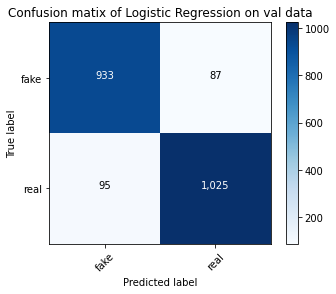
\includegraphics[width=0.4\linewidth]{logistic_regression.png}
\centering
\caption{Matrice di confusione per Logistic Regression}
\label{fig:bytepost}
\end{figure}

\subsection{Support Vector Machine}
Le Macchine a Vettori di Supporto o Macchine Kernel (Support Vector Machine, SVM) costituiscono un insieme di metodi di apprendimento supervisionato e possono essere utilizzate sia per fare Classificazione, sia per fare Regressione. SVM nasce come classificatore binario (2 classi), estendibile a più classi.
Date due classi di pattern multidimensionali linearmente separabili, tra tutti i possibili iperpiani di separazione, SVM determina quello in grado di separare le classi con il maggior margine possibile.
Il margine è la distanza minima di punti delle due classi nel training set dell'iperpiano individuato. 
La massimizzazione del margine è legata alla generalizzazione e se i pattern del training set sono classificati con ampio margine anche pattern del test set vicini al confine tra le classi saranno gestiti correttamente.
Il modello è stato addestrato sui dati di train e le prestazioni sono state valutate sul set di dati di val. \\
I risultati ottenuti sono i seguenti:
\begin{itemize}[noitemsep]
  \item \textbf{Accuracy}: 0.9317
  \item \textbf{Precison}: 0.9317
  \item \textbf{Recall}: 0.9317
  \item \textbf{F1}: 0.9317
 \end{itemize}

\noindent
La Figura 4 mostra la matrice di confusione ottenuta.
\begin{figure}[H]
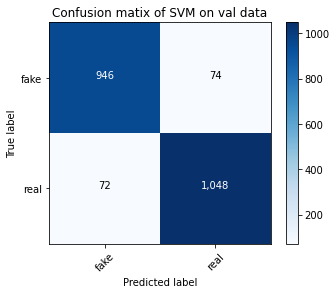
\includegraphics[width=0.5\linewidth]{SVM.png}
\centering
\caption{Matrice di confusione per Support Vector Machine}
\label{fig:bytepost}
\end{figure}

\subsection{Decision Tree Classifier}
Un albero decisionale è una struttura ad albero in cui un nodo rappresenta una caratteristica (o un attributo), il ramo rappresenta una regola decisionale e ogni nodo foglia rappresenta il risultato. Il nodo più in alto è il nodo radice. Un albero decisionale partiziona in base al valore dell'attributo (caratteristica) e viene partizionato in modo ricorsivo fino al raggiungimento dei nodi foglia. Sono molto utilizzati nei processi decisionali. Il modello è stato addestrato sui dati di train e le prestazioni sono state valutate sul set di dati di val. \\
I risultati ottenuti sono i seguenti:
\begin{itemize}[noitemsep]
  \item \textbf{Accuracy}: 0.8280
  \item \textbf{Precison}: 0.8281
  \item \textbf{Recall}: 0.8280
  \item \textbf{F1}: 0.8278
 \end{itemize}

\newpage
\noindent
La Figura 5 mostra la matrice di confusione ottenuta.
\begin{figure}[H]
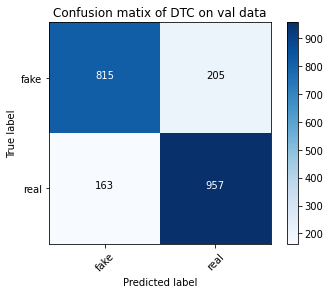
\includegraphics[width=0.5\linewidth]{DTC.png}
\centering
\caption{Matrice di confusione per Decision Tree Classifier}
\label{fig:bytepost}
\end{figure}

\subsection{Gradient Boost Classifier}
Gradient boosting è una tecnica di machine learning basata sull'un approccio di ensembles e può essere impiegata sia per la classificazione che per la regressione. Nel machine learning, l'ensembles è un approccio che combina più modelli di ML per creare un nuovo modello più complesso, che potenzialmente aggrega i benefici dei singoli modelli.
I singoli alberi sono modelli semplici (in ML sono spesso chiamati weak learners) che producono buone performance su alcune istanze dei dati. Gli alberi non sono profondi (tipicamente depth da 1 a 5), e questo rende il modello più compatto e veloce nelle predizioni. Il modello è stato addestrato sui dati di train e le prestazioni sono state valutate sul set di dati di val. \\
I risultati ottenuti sono i seguenti:
\begin{itemize}[noitemsep]
  \item \textbf{Accuracy}: 0.8565
  \item \textbf{Precison}: 0.8607
  \item \textbf{Recall}: 0.8565
  \item \textbf{F1}: 0.8565
 \end{itemize}

\noindent
La Figura 6 mostra la matrice di confusione ottenuta.
\begin{figure}[H]
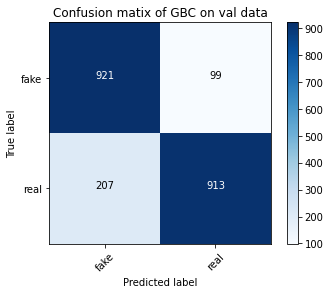
\includegraphics[width=0.5\linewidth]{GBC.png}
\centering
\caption{Matrice di confusione per Gradient Boost Classifier}
\label{fig:bytepost}
\end{figure}

\subsection{Rete Neurale - RNN}
Nel campo dell'apprendimento automatico, una rete neurale artificiale è un modello computazionale composto di "neuroni" artificiali, ispirato vagamente dalla semplificazione di una rete neurale biologica.
Un neurone riceve in ingresso segnali da vari altri neuroni tramite connessioni sinaptiche e li integra. Se l’attivazione che ne risulta supera una certa soglia genera un potenziale d’azione che si propaga attraverso il suo assone a uno o più neuroni. Possiamo considerare una rete neurale come una scatola nera, con degli input, degli strati intermedi in cui “succedono le cose”, e degli output che costituiscono il risultato finale. Esistono diverse tipologie di reti neurali e nel seguente caso è stata utilizzata una Recurrent Neural Network (RNN). Sono molto interessanti perchè, a differenza delle reti feed forward, in cui l’informazione può andare solo in un verso ed ogni neurone può essere interconnesso con uno o più neuroni della catena successiva, in questo tipo di reti, i neuroni  possono ammettere anche dei loop e/o possono essere interconnessi anche a neuroni di un precedente livello. \\
L'addestramento è stato eseguito su Google Colab dove sono stati caricati i file necessari e dove sono state definite le stesse funzioni utilizzate nel file \textit{fake-news-ml.ipynb} per il preprocessamento dei dati. Il notebook utilizzato su Colab è presente sempre nel repo GitHub (\textit{fake-news-RNN.ipynb}). Al suo interno per creare e addestrare il modello è stata utilizzata la libreria tensorflow. 
Nel seguente caso è stato generato un modello sequenziale contenente due livelli bidirezionali e tre livelli feed forward. I due livelli bidirezionali sono stati realizzati utilizzando reti neurali di tipo Long Short-Term Memory (LSTM). Le RNN funzionano ricordando informazioni precedenti e le utilizzano per elaborare l'input corrente ma hanno il difetto di non mantenere le dipendenze generate a lungo termine. Le LSTM sono state progettate proprio per evitare problemi di dipendenza a lungo termine e sono molto utilizzate per scopi relativi al riconoscimento del testo, alla traduzione automatica, al controllo di robot e molti altri.
Nei due livelli feed forward successivi sono stati utilizzati layer densi e ReLU come funzione di attivazione. In uscita ad ognuno di essi è stato inserito un livello Dropout, che spegne randomicamente un certo numero di unità del livello della rete e aiuta a prevenire overfitting. L'ultimo layer è quello di output.
Per addestrare la rete neurale è stata definita come loss function la Mean Squared Error, che misura il grado di accuratezza con cui la rete neurale riesce a descrivere i dati, e l'Accuracy come metrica da valutare durante l'addestramento. Nella funzione utilizzata per addestrare la rete neurale è stato dato in input anche il set di dati di validazione, utile per determinare i migliori iperparametri per la rete. Infine, il modello della rete neurale addestrata è stato utilizzato per valutare le prestazioni sul set di dati di test ed è stata ottenuta un'accuratezza pari a \textbf{0.9186}.

\noindent
La Figura 6 mostra la matrice di confusione ottenuta.
\begin{figure}[H]
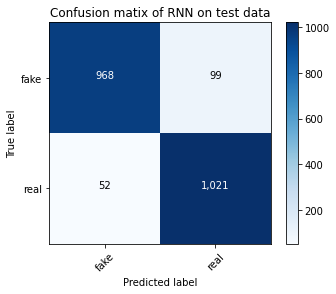
\includegraphics[width=0.5\linewidth]{RNN.png}
\centering
\caption{Matrice di confusione Rete Neurale - RNN}
\label{fig:bytepost}
\end{figure}


\subsection{Risultati}
Dai risultati ottenuti nelle precedenti sezioni è possibile osservare che il modello con accuratezza maggiore pari a \textit{0.9317} è la \textbf{SVM}, segue la Logistic Regression con accuratezza pari a \textit{0.9149} e il modello con accuratezza peggiore è il Decision Tree Classifier con \textit{0.8280}. \\
Il modello addestrato con maggiore accuratezza, in questo caso SVM, è stato testato anche sul set di dati di test ottenendo i seguenti risultati:
\begin{itemize}[noitemsep]
  \item \textbf{Accuracy}: 0.9364
  \item \textbf{Precison}: 0.9365
  \item \textbf{Recall}: 0.9364
  \item \textbf{F1}: 0.9364
 \end{itemize}

\noindent
La Figura 8 mostra la matrice di confusione ottenuta.
\begin{figure}[H]
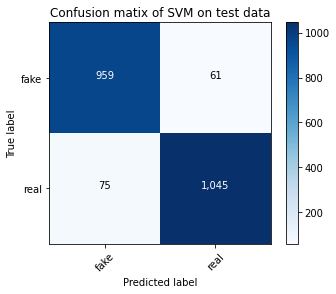
\includegraphics[width=0.5\linewidth]{SVM_test.png}
\centering
\caption{Matrice di confusione per Support Vector Machine sul test set}
\label{fig:bytepost}
\end{figure}

\noindent
Osservando i risultati anche sul set dei dati di test Support Vector Machine ottiene una maggiore accuratezza rispetto agli altri modelli e alla rete neurale RNN.

\newpage
\section{Conclusioni e sviluppi futuri}
In conclusione dai risultati ottenuti è possibile osservare che Support Vector Machine è il modello migliore con accuracy pari a \textit{0.9364} sul set di dati di test. Per quanto riguarda gli sviluppo futuri, si potrebbe arricchire il dataset collezionando nuovi dati multilingue e in tal caso introdurre tecniche deep learning più complesse.




\section{Riferimenti}
Patwa P. et al.: Fighting an Infodemic: COVID-19 Fake News Dataset. arXiv\\
preprint \href{https://arxiv.org/abs/2011.03327}{arXiv:2011.03327} (2020)




\end{document}